\documentclass[tikz,border=10pt]{standalone}
\usetikzlibrary{positioning}
\tikzset{main node/.style={circle,fill=blue!20,draw,minimum size=1cm,inner sep=0pt},
            }
\begin{document}
  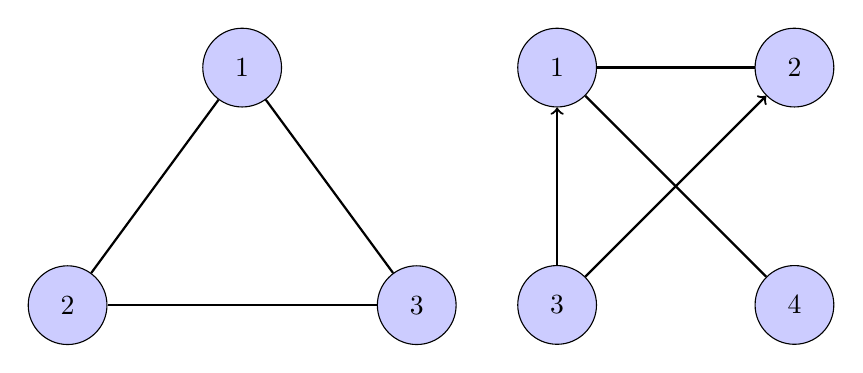
\begin{tikzpicture}
    \node[main node] (1) {$1$};
    \node[main node] (2) [below left = 2.3cm and 1.5cm of 1]  {$2$};
    \node[main node] (3) [below right = 2.3cm and 1.5cm of 1] {$3$};

    \path[draw,thick]
    (1) edge node {} (2)
    (2) edge node {} (3)
    (3) edge node {} (1);
    %%
    \begin{scope}[xshift=4cm]
    \node[main node] (1) {$1$};
    \node[main node] (2) [right = 2cm  of 1] {$2$};
    \node[main node] (3) [below = 2cm  of 1] {$3$};
    \node[main node] (4) [right = 2cm  of 3] {$4$};

    \path[draw,thick]
    (1) edge node {} (2)
    (1) edge node {} (4)
    (3) edge[->] node {} (2)
    (3) edge[->] node {} (1)
    ;
    \end{scope}
\end{tikzpicture}
\end{document}
